\begin{center}
\Huge
	Forberedelse til prøve
\end{center}

\subsection*{Opgave 1}
Bestem den afledede funktion til følgende funktioner:
\begin{align*}
	&1) \ 2x^2 + 10x^3 &&2) \ 5\sqrt{x} \\
	&3) \ \cos(x)-10 &&4) \ \ln(x)-\sqrt{7} \\
	&5) \ \textnormal{e}^{7}+\ln(4) &&6) \ -5x^{\frac{3}{2}} \\
\end{align*}

\subsection*{Opgave 2}
Bestem den afledte funktion til følgende funktioner:
\begin{align*}
	&1) \ \ln(x^2+11x-6) &&2) \ \cos(x)\cdot(4x^2-3x^5) \\
	&3) \  8\sqrt{x}\cdot \textnormal{e}^{x} &&4) \ \textnormal{e}^{4\sin(x)}\\
	&5) \ 2^{5x+11} &&6) \ \frac{x^{\frac{1}{2}}}{-2\ln(x)} \\
\end{align*}

\newpage

\subsection*{Opgave 3}

\begin{enumerate}[label=\roman*)]
	\item En funktion $f$ er givet ved
	\begin{align*}
		f(t) = 6t^2-11t+7.
	\end{align*}
	Bestem tangenthældningen til $t = 4$.
	\item En funktion $g$ er givet ved
	\begin{align*}
		g(x) = \ln(x)+4x.
	\end{align*}
	Bestem tangenthældningen for grafen for $g$ i punktet $(1,g(1))$.
	\item En funktion $h$ er givet ved
	\begin{align*}
		h(x) = x^2-4x+11.
	\end{align*}
	Bestem det sted, hvor tangenthældningen for grafen for $h$ er 2.
	
\end{enumerate}

\subsection*{Opgave 4}

\begin{enumerate}[label=\roman*)]
	\item En funktion $f$ er givet ved
	\begin{align*}
		f(t) = t^3 - 3t^2 + 4.
	\end{align*}
	Bestem de steder, hvor $f$ har ekstrema.
	\item En funktion $g$ er givet ved
	\begin{align*}
		g(x) = \ln(x)+2\sqrt{x}+4
	\end{align*}
	Bestem ligningen for tangenten til grafen for $g$ gennem punktet $(1,g(1))$. 
	\item En funktion $h$ er givet ved
	\begin{align*}
		h(x) = \cos(x)\cdot(6x^2+4x+7).
	\end{align*}
	Bestem $h'(0)$.

\end{enumerate}

\subsection*{Opgave 5}

\begin{enumerate}[label=\roman*)]
	\item En funktion $f$ er givet ved
	\begin{align*}
		f(x) = x^3 + 3x^2 - 4x + k.
	\end{align*}
	Bestem de værdier for $k$, så $f$ har linjen med ligningen $y = 16x-10$ som tangent
	\item En funktion $h$ er givet ved
	\begin{align*}
		h(x) = x^3-3x^2+3x+4.
	\end{align*}
	Bestem tallet $a$, så ligningen $h'(x) = a$ har så få løsninger som muligt.
\end{enumerate}

\subsection*{Opgave 6}
Bestem hvilke af graferne der tilsvarer funktionen $f$ og hvilken der tilsvarer $f'$
\begin{center}

\scalebox{0.6}{
	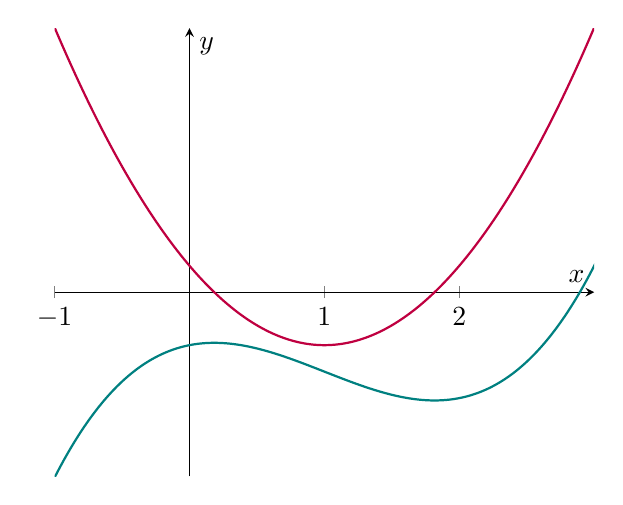
\begin{tikzpicture}
		\begin{axis}[axis lines = middle, xmin = -1, xmax = 3, xtick = {-1,1,2}, ytick = {0},
		xlabel = $x$, 
		ylabel = $y$]
			\addplot[samples = 1000, color = teal, thick] {x^3-3*x^2+x-2};
			\addplot[samples = 1000, color = purple, thick] {3*x^2-6*x+1};
		\end{axis}
	\end{tikzpicture}
	}
	\qquad
\scalebox{0.6}{
	\begin{tikzpicture}
		\begin{axis}[axis lines = middle, xmin = 0.1, xmax = 2, xtick = {1}, ytick = {0},
		xlabel = $x$, 
		ylabel = $y$]
			\addplot[samples = 1000, color = teal, thick] {1/x - 2*x};
			\addplot[samples = 1000, color = purple, thick] {ln(x)-x^2};
		\end{axis}
	\end{tikzpicture}
}

\scalebox{0.6}{
	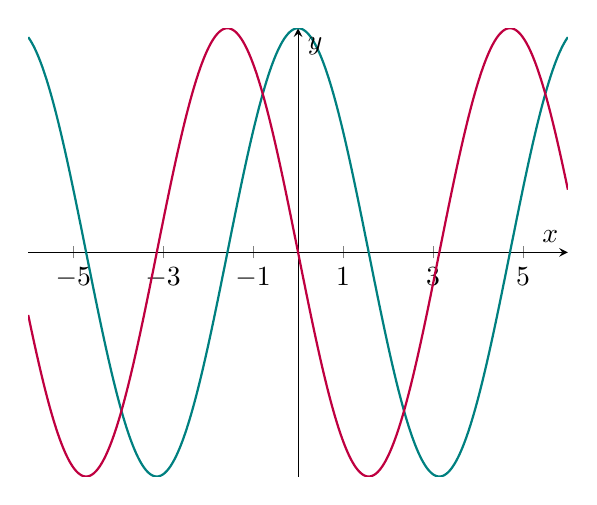
\begin{tikzpicture}
		\begin{axis}[axis lines = middle, xmin = -6, xmax = 6, xtick = {-5,-3,-1,1,3,5}, ytick = {0},
		xlabel = $x$, 
		ylabel = $y$]
			\addplot[samples = 1000, color = teal, thick, domain = -6:6] {cos(deg(x))};
			\addplot[samples = 1000, color = purple, thick, domain = -6:6] {-sin(deg(x))};
		\end{axis}
	\end{tikzpicture}
	}
	\qquad
\scalebox{0.6}{
	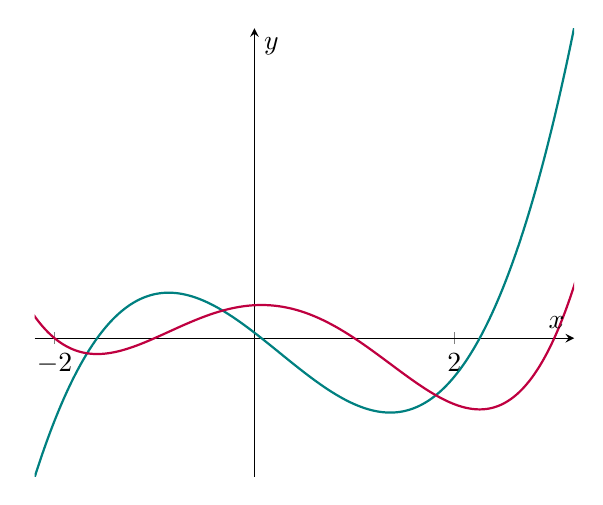
\begin{tikzpicture}
		\begin{axis}[axis lines = middle, xmin = -2.2, xmax = 3.2, xtick = {-2,2}, ytick = {0},
		xlabel = $x$, 
		ylabel = $y$]
			\addplot[samples = 1000, color = teal, thick] {4*x^3-3*x^2-14*x+1};
			\addplot[samples = 1000, color = purple, thick] {(x-1)*(x-3)*(x+1)*(x+2)};
		\end{axis}
	\end{tikzpicture}
}
\end{center}

\subsection*{Opgave 7}

\begin{enumerate}[label=\roman*)]
	\item For en funktion $g$ gælder der, at $g'(x) = 0$ hvis og kun hvis $x = 2$ eller $x = 4$ samt at $g'(-4) = 1$, $g'(3) = 2$ og $g'(5) = -2$.   
	Opskriv monotoniforholdene for $g$	
	\item Bestem monotoniforholdene for funktionen $f$ givet ved
	\begin{align*}
		f(x) = x^2 -x - 2
	\end{align*}
	\item Bestem monotoniforholdene for funktionen $g$ givet ved
	\begin{align*}
		x^3 - 3x^2 + 3x + 10
	\end{align*}

\end{enumerate}
\newpage

\subsection*{Opgave 8}
\begin{enumerate}[label = \roman*)]
	\item En funktion $f$ er givet ved
	\begin{align*}
		f(x) = 2x^2 + 4.
	\end{align*}
	Brug definitionen for differentialkvotienten til at vise, at $f'(2) = 16$. 
	\item En funktion $g$ er givet ved
	\begin{align*}
		g(x) = \frac{1}{2+x}
	\end{align*}
	Brug definitionen for differentialkvotienten til at vise, at $f'(3) = -\frac{1}{25}$.
\end{enumerate}